\documentclass[a4paper,10]{article}
\usepackage[utf8]{inputenc}
\usepackage{url}
\usepackage[pdftex]{graphics}
\usepackage{graphicx} 
%\usepackage{tikz}
%\usepackage{natbib}
%\usepackage[symbol]{footmisc}
%\usepackage{t1pl}
\usepackage[T1]{fontenc} 
%\usepackage{subfigure}
\usepackage{amsmath}
\usepackage{amssymb}

\usepackage[polish]{babel}
\selectlanguage{polish}

\usepackage{xcolor}

\usepackage{hyperref}

\newcommand{\comment}[2]{\noindent{{\scriptsize\sffamily(\marginpar{\sffamily #1}#2)}}}
\newcommand{\jw}[1]{\comment{\tiny{JW}}{\textcolor{blue}{#1}}}
\newcommand{\amcol}[1]{\textcolor{blue}{#1}}
\newcommand{\am}[1]{\comment{\tiny AM}{\textcolor{orange}{#1}}}

\DeclareMathOperator*{\argmax}{arg\,max}

% \title{Opis metody CRF przystosowanej do \\ujednoznaczniania morfoskładniowego}
\title{Opis narzędzia do\\ ujednoznaczniania morfoskładniowego\\ opartego na formaliźmie\\ \emph{Conditional Random Fields}}

\author{Jakub Waszczuk}

% \address{Institute of Computer Science, Polish Academy of Sciences\\
%               J. K. Ordona 21, 01-237 Warsaw, Poland
% }
%\abstract{

%%%%%%%%%%%%%%%%%%%%%%%%%%%%%%%%%%%%%%%%%%%%%%%%%%%%%%%%%%%%%%%%%%%%%%

\begin{document}

\bibliographystyle{plain}

\maketitle

\tableofcontents

\clearpage

\section{Wprowadzenie}

Dokument opisuje narzędzie służące do ujednoznaczniania morfoskładniowego (tager) 
bazujące na probabilistycznym formaliźmie \emph{Conditional Random Fields}.
W pierwszym rozdziale opiszemy ogólny zarys działania narzędzia oraz przepływ
danych pomiędzy jego komponentami. Szczegóły na temat działania poszczególnych
modułów zostaną podane w kolejnych rozdziałach.

Na początek wprowadzimy podstawowe pojęcia niezbędne do zrozumienia
działania tagera, którego na tym etapie będziemy traktować jak czarną skrzynkę.
Przez \emph{zdanie} będziemy rozumieli, zgodnie z potocznym rozumieniem tego
słowa, sekwencję \emph{słów}. Ponieważ poruszamy się w temacie oznaczania
morfoskładniowego, zakładamy że z każdym słowem powiązany jest zestaw
\emph{interpretacji morfoskładniowych} ustalony na etapie analizy morfoskładniowej.
Każda interpretacja morfoskładniowa reprezentowana jest przez dwa komponenty:
\begin{itemize}
\item Leksem (reprezentowany przez swoją formę podstawową), którego słowo
w tekście jest wykładnikiem,
\item Napis powstały przez sklejenie informacji o części mowy oraz wartościach
kategorii gramatycznych. Napis ten będziemy nazywać \emph{znacznikiem} lub \emph{etykietą}.
\end{itemize}
W ogólnym przypadku, celem ujednoznaczniania jest określenie, m. in. na podstawie
kontekstów, poprawnych interpretacji morfoskładniowych poszczególnych
słów (w wyniku czego każdemu słowu przypisany zostaje dokładnie jeden
leksem i znacznik).
My będziemy ograniczać się jedynie do ujednoznaczniania na poziomie znaczników,
czyli wyboru poprawnych interpretacji gramatycznych (wartości częsci mowy i kategorii
gramatycznych) poszczególnych słów.
W konsekwencji, proces ujednoznaczniania który będziemy opisywać w dalszej
części tego dokumentu może prowadzić do wyboru kilku interpretacji
morfoskładniowych dla niektórych słów w zdaniu (ale każda z tych interpretacji
będzie identyczna na poziomie gramatycznym, czyli będzie powiązana z takim
samym znacznikiem).

Ważnym etapem ujednoznaczniania jest określenie \emph{obserwacji} poszczególnych
słów. To obserwacje służą do reprezentowania słowa na poziomie modelu
\emph{Conditional Random Field} (CRF) -- w trakcie trenowania tagera
określane są statystyczne relacje pomiędzy etykietami określonymi
dla zadanego słowa a jego obserwacjami (określane są również relacje
pomiędzy sąsiadującymi etykietami, ale o tym później). Przykładowe obserwacje to:
forma ortograficzna słowa (czyli słowo w swojej oryginalnej postaci),
słowo poprzednie, słowo następne (lub słowo z dalszego kontekstu),
a także prefiksy (pierwsze $k$ znaków) lub sufiksy (ostatnie $k$ znaków)
formy ortograficznej. Obecna implementacja nie uwzględnia obserwacji
innego typu, ale ich dodanie -- jeśli okaże się potrzebne -- nie powinno być trudne.
Testy różnych konfiguracji tagera wykazały, że
uwzględnianie słów z kontekstu ma istotny wpływ na jakość wyników ujednoznaczniania. 
Przykładowo, w modelu wytrenowanym  w fazie wstępnych testów tagera
znaleziona została następująca zależność: jeśli forma ortograficzna
poprzedniego słowa jest równa ,,jest'', to jest bardzo mało prawdopodobne,
że bierzące słowo jest przymiotnikiem w bierniku.
Więcej informacji na temat określania obserwacji poszczególnych
słów można znaleźć w rozdziale \ref{sec:schema_def}. 

Poza relacjami obserwacja-etykieta tager modeluje również relacje występujące
na poziomie etykiet. Etykiety są jednak najpierw poddawane procesowi dzielenia
na warstwy, dokładniej opisanemu w rozdziale \ref{sec:layers}.
Znaczniki morfoskładniowe składają się z wielu
części reprezentujących wartości części mowy oraz różnych kategorii gramatycznych.
Znaczniki są dzielone ze względu na typy kategorii i przenoszone do osobnych
warstw znakowania. Przykładowy podział może wyglądać następująco:
części mowy, przypadki oraz osoby trafiają do pierwszej warstwy,
natomiast wartości pozostałych kategorii gramatycznych do drugiej.
% (możliwe jest też zdefiniowanie podziału na większą liczbę warstw).
Weźmy przykładowe słowo ,,bez'', dla którego analiza morfoskłaniowa daje
[prep:gen:nwok, subst:pl:gen:f, subst:sg:acc:m3, subst:sg:nom:m3]
(znaczniki przedstawione sa w formacie NKJP).
Po przeprowadzeniu opisanego powyżej podziału każdy znacznik będzie miał postać pary,
z pierwszym elementem reprezentującym wartości cześci mowy, przypadka i osoby, a drugim
-- wartości pozostałych kategorii. Tak więc wynik podziału będzie następujący:
[(prep:gen, nwok), (subst:gen, pl:f), (subst:acc, sg:m3), (subst:nom, sg:m3)].
Tager modeluje relacje między trzema kolejnymi pod-etykietami osobno
dla każdej warstwy znakowania. Tak więc, jeśli w pierwszej warstwie będą
wyłącznie części mowy, a w drugiej wyłącznie przypadki, to tager osobno
będzie modelował relacje między sąsiadującymi ze sobą częściamy mowy,
a osobno między sąsiadującymi wartościami przypadku. Ponadto, wartości
obserwacji określane są osobno nie tylko dla każdego słowa, ale także
dla każdej warstwy niezależnie. Tager nie zabrania jednak zdefiniowania
takich samych typów obserwacji dla różnych warstw oznaczania.
Nie zabrania także przepisywania wartości jednej kategorii (podczas podziału
znaczników na warstwy) do kilku różnych warstw.
Sposób podziału znaczników na warstwy definiowany jest w pliku konfiguracyjnym 
tagera. Więcej informacji na ten temat można znaleźć w rozdziale \ref{sec:schema_def}.

\begin{figure}[ht]
\begin{center}
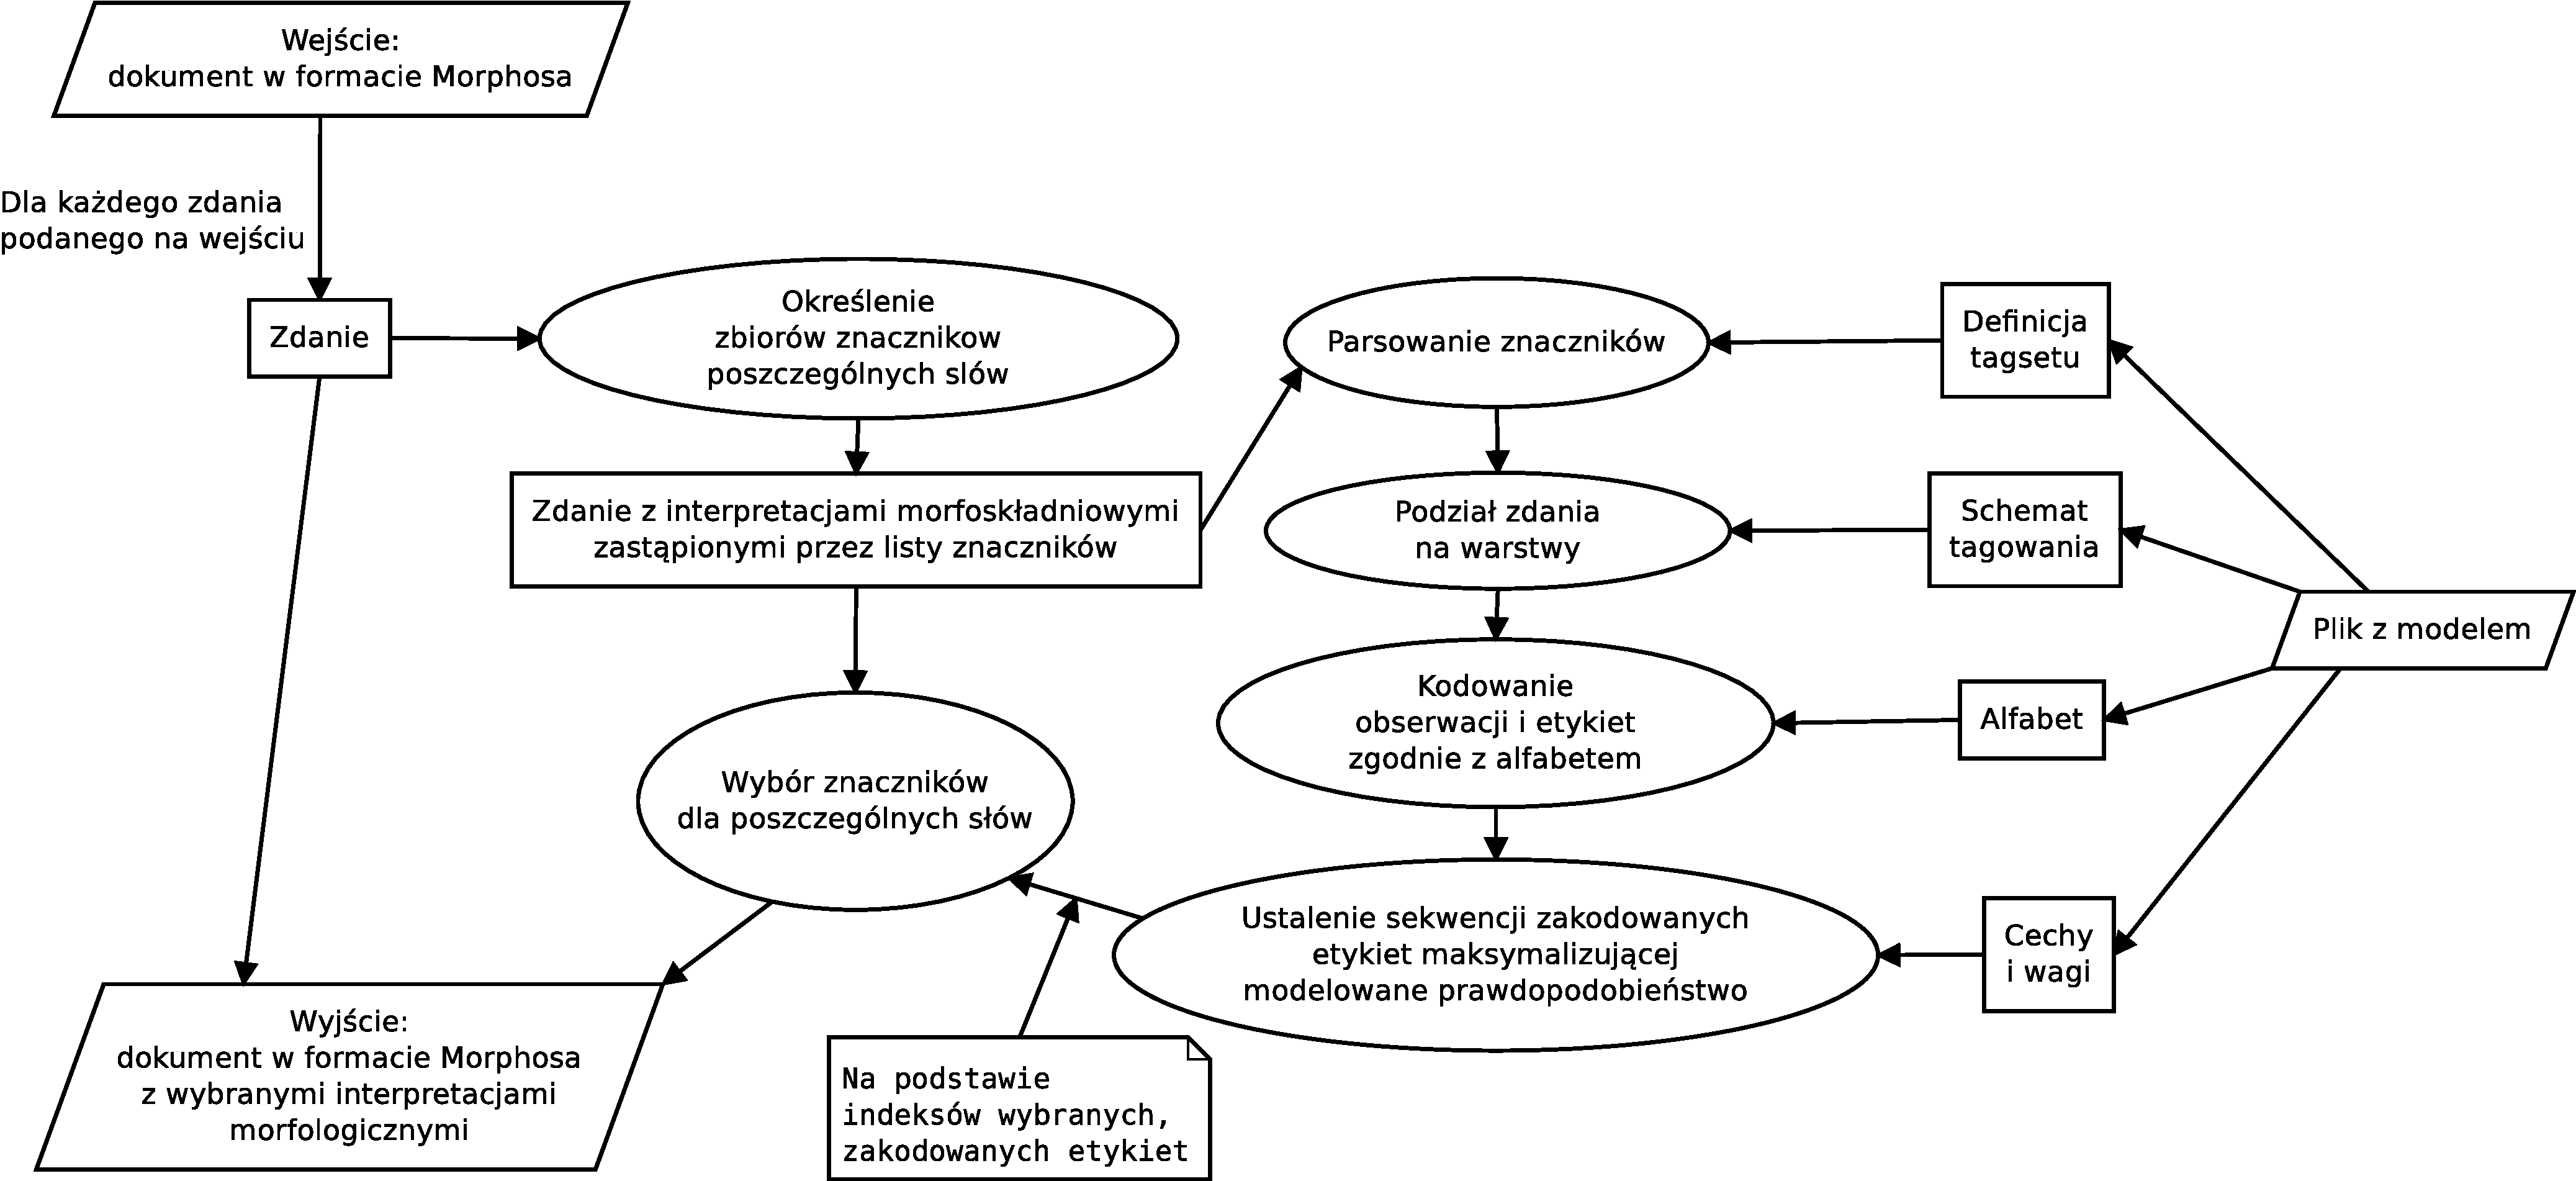
\includegraphics[width=1.0\textwidth]{tag-flow.pdf}
 \caption{Diagram przepływu danych w procesie ujednoznaczniania}\label{rys:tag-flow}
\end{center}
\end{figure}

Przepływ danych w trakcie ujednoznaczniania zbioru zdań wzbogaconych dodatkowymi informacjami
o możliwych interpretacjach morfoskładniowych poszczególnych słów przedstawiony jest
na rysunku \ref{rys:tag-flow}.
Na samym początku wczytywany jest w całości do pamięci, zapisany na dysku w postaci
binarnej, model składający się z czterech komponentów. Na pierwszy z nich składają
się cechy modelu wraz z odpowiadającymi im wagami, czyli właściwy model CRF.
% W pliku z modelem znajduje się lista cech wraz z przypisanymi im wagami.
% Każda z cech stanowi krotkę liczb całkowitych, które otrzymywane są
% z właściwych wartości obserwacji i etykiet w trakcie ich tłumaczenia
% na podstawie alfabetu. 
Drugim elementem jest \emph{alfabet}, który stanowi zbiór map służących
do tłumaczenia obserwacji i etykiet (które na wejściu mają postać
napisów) na liczby całkowite, które będą reprezentować je w dalszej części
procesu ujednoznaczniania. Zabieg ten ma zmiejszyć wymagania pamięciowe
narzędzia i przyszpieszyć cały proces.
Więcej informacji na ten temat można znaleźć w rozdziale \ref{sec:model_repr}. 
Kolejnym komponentem modelu jest \emph{definicja tagsetu}, która pozwala parsować i
poprawnie interpretować znaczniki gramatyczne. Dzięki temu możliwe
jest sprawdzanie poprawności znaczników (czy są zgodne z regułami
podanymi w definicji tagsetu) oraz ich ,,rozbijanie'' na poszczególne
warstwy ujednoznaczniania. Ta druga czynność jest możliwa, ponieważ w definicji
tagsetu podane są również informacje o zbiorach wartości przyjmowanych
przez poszczególne kategorie gramatyczne. 
%\item Wczytywany jest opis tagsetu. Tagset służy tagerowi do ,,rozbijania''
%znaczników na poszczególne pola -- części mowy i wartości kategorii gramatycznych
%-- dzięki czemu mogą być one później dzielone między różne warstwy tagowania.
Więcej na temat definiowania tagsetu można znaleźć w rozdziale \ref{sec:tag_def}.
Ostatnim elementem jest \emph{schemat tagowania}, główny plik konfiguracyjny tagera. 
W pliku tym zdefiniowane są reguły podziału na poszczególne warstwy oznaczania
oraz grupy obserwacji. Więcej na temat definiowania schematu można znaleźć
w rozdziale \ref{sec:schema_def}.

Po wczytaniu całego modelu rozpoczyna się proces ujednoznaczniania.
Wczytywany jest -- ze standardowego wejścia lub z podanego jako argument
pliku -- dokument w formacie Morphosa (możliwe jest również
ujednoznacznianie pliku wejściowego w wewnętrznym formacie narzędzia
o nazwie LINC -- opis tego formatu można znaleźć w rozdziale
\ref{sec:linc_format}).
Przez format Morphosa rozumiemy tutaj format wyjściowy analizatora Morphos
przeznaczony do dalszego ujednoznaczniania.
Dokument wejściowy jest dzielony na zdania, zgodnie z identyfikatorami zdań,
a następnie każde ze zdań poddawane jest niezależnie procesowi
ujednoznaczniania.
% \jw{TODO: ponieważ poszczególne zdania przetwarzane są niezależnie,
Każde ze zdań należących do zbioru wejściowego przetwarzane jest w następujący sposób:
\begin{itemize}
\item Dla każdego słowa określany jest zbiór potencjalnych znaczników.
  W wejściowym pliku w formacie Morphosa dla każdego słowa podane są
  wszystkie jego interpretacje morfoskładniowe. Jak już wcześniej
  wspomnieliśmy, wśród tych interpretacji niektóre znaczniki mogą
  się powtarzać, dlatego otrzymany zbiór znaczników może być mniejszy
  niż zbiór interpretacji morfoskładniowych.
\item Znaczniki występujące w zdaniu są parsowane zgodnie
  z definicją tagsetu.
\item Zdanie zostaje podzielone na warstwy, zgodnie ze schematem ujednoznaczniania.
  Dla każdego słowa określane są obserwacje należące do poszczególnych
  warstw oznaczania.
  Poszczególne znaczniki, sparsowane w poprzednim kroku, dzielone są pomiędzy
  poszczególne warstwy oznaczania.
\item Obserwacje tłumaczone są, przy pomocy alfabetu obserwacji, na liczby całkowite.
  Wartości nie znalezione w alfabecie są ignorowane.
  Pod-etykiety (przez pod-etykietę rozumiemy tutaj połączone części pełnego znacznika,
  które trafiły do tej samej warstwy) tłumaczone są na
  liczby całkowite przy pomocy alfabetów etykiet (dla każdej warstwy zdefiniowany
  jest osobny alfabet).
  Etykieta, która nie wystąpiła w odpowiednim alfabecie, otrzymuje numer
  $-1$ (wartość nie występująca w żadnym alfabecie) -- taka sytuacja jest skrajna
  i nie powinna wystepować.
\item Algorytm opisany w rozdziale \ref{sec:disamb} zastosowany jest do
  określenia najbardziej prawdopodobnej sekwencji znaczników. Dokładniej,
  dla każdego słowa określony zostaje indeks wybranego znacznika i na tej
  podstawie określane są wybrane interpretacje morfoskładniowe w zbiorze
  wejściowym. Wybrany znacznik może pojawiać się
  przy kilku interpretacjach słowa w zbiorze tekstowym -- wtedy każda
  z tych interpretacji zostanie oznaczona jako wybrana.
\end{itemize}

Opisany powyżej proces dotyczy sytuacji ujednoznaczniania, czyli procesu w którym
dla każdego słowa wybrany zostaje dokładnie jeden znacznik.
Narzędzie można uruchomić również w trybie, w którym do każdego
z potencjalnych znaczników przypisane jest jego prawdopodobieństwo,
zgodnie z wytrenowanym modelem. Zachowana jest własność, że znacznik, który
zostałby wybrany w procesie ujednoznaczniania, otrzymuje najwyższe
prawdopodobieństwo. Algorytm przypisywania prawdopodobieństw
również opisany jest w rozdziale \ref{sec:tag_probs}.
W sytuacji, gdy identyczny znacznik występuje w dwóch lub więcej
interpretacjach morfoskładniowych formy ortograficznej występującej
w tekście, prawdopodobieństwa poszczególnych interpretacji są
ponownie normalizowane.

\section{Conditional Random Fields}

\subsection{Oznaczenia}

\begin{itemize}
\item $O$ -- Zbiór wszystkich \emph{obserwacji}.
\item $Y$ -- Zbiór wszystkich \emph{etykiet} (lub \emph{znaczników}),
rozszerzony o specjalną etykietę $\gamma$ przypisywaną niedodatnim
pozycjom w zdaniu.
\item $x = \lbrace x_i \rbrace_{i=1}^n$ -- \emph{Zdanie},
czyli ciąg \emph{słów} długości $n$. 
Każde słowo $x_i$ reprezentowane jest przez zbiór obserwacji
$\lbrace o_1, o_2, \ldots \rbrace$, $o_i \in O$, określonych dla $i$-tej
pozycji w zdaniu. Typowe obserwacje to: forma ortograficzna
$i$-tego słowa, formy ortograficzne sąsiednich słów, prefiksy i sufiksy
form ortograficznych itd. Obserwacje brane pod uwagę podczas trenowania
i ujednoznaczniania określane są na podstawie pliku konfiguracyjnego tagera.
\item $y = \lbrace y_i \rbrace_{i=-1}^n$ -- Ciąg etykiet
przypisanych poszczególnym słowom zdania.
Dla $i \geq 1$ mamy $y_i \in Y \setminus \lbrace \gamma \rbrace$
oraz $y_i = \gamma$ dla $i < 1$.
\item $r = \lbrace r_i \rbrace_{i=-1}^n$ -- Ciąg \emph{ograniczeń}
na etykiety na poszczególnych pozycjach w zdaniu.
Symbol $r_i$ reprezentuje zbiór etykiet, które może
przyjąć słowo na $i$-tej pozycji w zdaniu.
W kontekście ujednoznaczniania, $r_i$ reprezentuje
wynik analizy morfoskładniowej $i$-tego słowa.
Dla $i \geq 1$ mamy $r_i \subseteq Y \setminus \lbrace \gamma \rbrace$
oraz $r_i = \lbrace \gamma \rbrace$ dla $i < 1$.
\item Zdanie $x$ będziemy nazywać również \emph{nieoznakowanym zdaniem},
natomiast parę $(x, y)$ będziemy nazywać \emph{oznakowanym zdaniem},
jeśli każdej pozycji $i$ zdania $x$ przypisana została etykieta $y_i$.
Alternatywnie, gdy będziemy chcieli podkreślić ograniczenia na poszczególne
pozycje w zdaniu, \emph{nieoznakowanym zdaniem} będziemy nazywali parę $(x, r)$,
a trójkę $(x, y, r)$ -- \emph{oznakowanym zdaniem}, o ile na każdej pozycji $i$
zdania $x$ przypisana została etykieta $y_i$ oraz $y_i \in r_i$.
\item $F$ -- Zbiór \emph{cech} modelu CRF. 
Na początek założymy, że cechy modelu przyjmują jedną z dwóch postaci:
$(u, v, w)$ lub $(o, u)$,
przy czym $o \in O$ stanowi obserwację, natomiast $u, v, w \in Y$ są etykietami
odpowiadającymi odpowiednio: aktualnej, poprzedniej i przed-poprzedniej
pozycji w zdaniu\footnote{Tak skonstruowany model można nazwać modelem drugiego
rzędu, ponieważ cechy modelu postaci $(u, v, w)$ uwględniają trzy następujące
po sobie etykiety.}.
Cechy $(u, v, w)$ odpowiadają za modelowanie relacji między sąsiednimi
etykietami, natomiast $(o, u)$ -- za modelowanie relacji między obserwacjami
a etykietami określonymi względem tych samych pozycji w zdaniu.
Postać cech modelu zostanie niecho zmieniona w rozdziale \ref{sec:layers}.
\item $f_k(y, x, i)$ -- Binarna funkcja $f$ przyjmująca wartość 1
wtedy i tylko wtedy, gdy $k$-ta cecha modelu spełniona jest
na $i$-tej pozycji zdania $(x, y)$.
Powiemy, że $k$-ta cecha modelu postaci $(u, v, w)$ jest spełniona na $i$-tej
pozycji oznakowanego zdania $(x, y)$,
jeśli etykiety $u, v, w$ są równe etykietom na odpowiednich pozycjach w zdaniu,
czyli $u = y_i$, $v = y_{i-1}$ oraz $w = y_{i-2}$.
Analogicznie, cecha modelu postaci $(o, u)$ jest spełniona na $i$-tej
pozycji oznakowanego zdania $(x, y)$, jeśli obserwacja $o$ należy do
zbioru obserwacji określonej dla $i$-tej pozycji zdania oraz $u = y_i$.
\item $\Lambda = \lbrace \lambda_k \rbrace_{k=1}^{|F|}$ -- \emph{Parametry}
modelu CRF. Parametr $k$-ty określna wagę $k$-tej cechy modelu
(zob. wzór \ref{traditional_crf}).
\item $M = (F, f, \Lambda)$ -- Model CRF określony przez zbiór cech $F$,
binarną funckja $f$ oraz zbiór parametrów $\Lambda$.
\item $p$ -- Rozkład prawdopodobieństwa określony przez model CRF.
\end{itemize}

\subsection{Definicja}

Niech $x$ będzie zdaniem długości $n$ oraz $y$ oznacza ciąg etykiet
długości $n$.
Tradycyjny model CRF ($F$, $f$, $\Lambda$) definiuje
warunkowe prawdopodobieństwo $p(y \vert x, \Lambda)$
zgodnie ze wzorem:
\begin{equation}\label{traditional_crf}
p(y \vert x, \Lambda) = \frac{1}{Z(x, \Lambda)} \exp 
\left( \sum_{i, k} f_k(y, x, i) \lambda_k \right)
\end{equation}
gdzie $f_k(y, x, i)$ to binarna funkcja przyjmująca wartość 1
wtedy i tylko wtedy, gdy $k$-ta cecha modelu spełniona jest
na $i$-tej pozycji oznakowanego zdania $(x, y)$,
$\lambda_k$ jest $k$-tym parametrem modelu, 
a funkcja $Z(x, \Lambda)$ (odpowiadająca za normalizację prawdopodobieństwa)
zdefiniowana jest wzorem:
\begin{equation}
Z(x, \Lambda) = \sum_{y^\prime \in (Y \setminus \lbrace \gamma \rbrace)^n} \exp
\left( \sum_{i, k} f_k(y^\prime, x, i) \lambda_k \right)
\end{equation}

\subsection{Wykorzystanie wyników analizy morfoskładniowej}

Tradycyjny model CRF nie wykorzystuje dodatkowych informacji
uzyskanych na etapie analizy morfoskładniowej.
Zgodnie z takim modelem, na każdej pozycji zdania $x$ może zostać przypisana
dowolna (poza $\gamma$) etykieta ze zbioru $Y$.

Analiza pozwala określić zbiory dopuszczalnych znaczników
na poszczególnych pozycjach zdania. Podamy teraz zmodyfikowaną
wersję CRFs, która uwzględnia te dodatkowe informacje.
%Podamy teraz zmodyfikowaną definicję modelu CRF, która wykorzystuje wyjściowe
%informacje analizy morfoskładniowej.
Niech $x$ będzie zdaniem długości $n$, $y$ oznacza ciąg etykiet
długości $n$ oraz $r$ oznacza ograniczenia na wartości etykiet na poszczególnych
pozycjach zdania $x$.
Prawdopodobieństwo warunkowe $p(y \vert x, r, \Lambda)$ zdefiniujemy następująco:

\begin{equation}\label{restricted_crf}
p(y \vert x, r, \Lambda) = \left\{
 \begin{array}{cl}
  0 & \mbox{jeśli } y \notin \prod_i r_i\\
  \frac{1}{Z(x, r, \Lambda)} \exp \left( \sum_{i, k} f_k(y, x, i)
  \lambda_k \right) & \mbox{wpp.}
 \end{array} \right.
\end{equation}

Jeśli sekwencja etykiet $y$ nie jest zgodna z zestawem ograniczeń
(dla pewnego $i$, etykieta przypisana do $i$-tego słowa w zdaniu
nie należy do zbioru interpretacji tego słowa określonego na etapie analizy),
to modelowane prawdopodobieństwo jest równe $0$.
W przeciwnym razie prawdopodobieństwo obliczane jest tak jak wcześniej,
z tą różnicą, że wyliczenie składnika normalizującego $Z(x, r, \Lambda)$ sprowadza się
do sumowania wyłącznie po poprawnych (zgodnych z ograniczeniami)
sekwencjach etykiet:

\begin{equation}
Z(x, r, \Lambda) = \sum_{y^\prime \in \prod_i r_i} \exp
\left( \sum_{i, k} f_k(y^\prime, x, i) \lambda_k \right)
\end{equation}

\subsection{Podział na warstwy}\label{sec:layers}

W zastosowaniu opisywanej metody do ujednoznaczniania
morfoskładniowego liczba różnych znaczników (rozmiar zbioru $Y$)
może być większa niż $10^3$. 
W związku z tym liczba cech modelu, mimo że ograniczona do cech
występujących w zbiorze treningowym, może być bardzo duża (jeśli przyjmiemy,
że liczba różnych znaczników jest równa $10^3$, to liczba wszystkich
możliwych cech modelu postaci $(u, v, w)$ wynosi $10^9$).

W celu ograniczenia liczby parametrów oraz poprawienia jakości modelu
wprowadziliśmy kolejną modyfikacje formalizmu CRFs. Etykiety, a jednocześnie
znaczniki  morfoskładniowe, składają się z wielu części reprezentujących
wartości części mowy oraz różnych kategorii gramatycznych.
Znaczniki są dzielone ze względu na typy kategorii i przenoszone
do osobnych warstw znakowania.
Fragmenty, które trafiły do tej samej warstwy, sklejane są w jedną
\emph{pod-etykietę} (lub \emph{pod-znacznik}).
Przykładowy podział może być następujący:
części mowy, przypadki oraz osoby trafiają do pierwszej warstwy,
natomiast wartości pozostałych kategorii gramatycznych do
drugiej\footnote{Takie rozwiązanie zostało zainspirowane narzędziem Pantera,
w którym ujednoznacznianie odbywa się wieloprzebiegowo.}. 
Sposób podziału specyfikuje się w pliku konfiguracyjnym
tagera\footnote{Konfiguracja nie wyklucza przepisania wartości
wybranego atrybutu -- np. części mowy -- do kilku warstw.}.

W efekcie podziału otrzymujemy $L$ warstw o numerach $1, \ldots, L$.
Ciąg etykiet $y$ obcięty do $l$-tej warstwy
(czyli ciąg pod-etykiet otrzymanych poprzez sklejenie przepisanych do $l$-tej
warstwy informacji na każdej pozycji zdania)
będziemy oznaczać przez $y^{(j)}$, a zbiory wszystkich pod-etykiet występujących
w kolejnych warstwach -- przez $Y_1, Y_2, \ldots, Y_L$.
Podział znaczników będziemy opisywać przy pomocy rodziny funkcji
$\delta_l: Y \rightarrow Y_l$, gdzie $\delta_l$ reprezentuje funckje
wycinającą z zadanego znacznika $y$ część należącą do $l$-tej warstwy.
Analogicznie, ciąg słów obcięty do $l$-tej warstwy\footnote{Konfiguracja pozwala
na definiowanie różnych typów obserwacji dla różnych warstw.} będziemy
oznaczać przez $x^{(j)}$, a ciąg ograniczeń obcięty do $l$-tej warstwy
-- $i$-tym elementem ciągu będzie zbiór $\lbrace \delta_j(y) : y \in
r_i \rbrace$ -- przez $r^{(j)}$.
Definiujemy charakterystyczne dla poszczególnych warstw cechy
modelu CRF, które przyjmują jedną z dwóch postaci:
$(l, u, v, w)$ lub $(l, o, u)$, gdzie $l$
reprezentuje numer warstwy, $o$ -- określoną dla $l$-tej warstwy
obserwację, natomiast $u, v, w \in Y_l$ są należącymi do $l$-tej
warstwy etykietami przypisanymi odpowiednio do:
aktualnej, poprzedniej i przed-poprzedniej pozycji w zdaniu.

Binarną funkcję $f$ definiujemy tym razem względem zadanej
warstwy o numerze $j$.
Niech $k$-ta cecha modelu ma postać $(l, u, v, w)$.
Funkcja $f_k(y, x, i, j)$ przyjmuje wartość 1 (co oznacza, że $k$-ta cecha modelu
jest spełniona w $j$-tej warstwie na $i$-tej pozycji oznakowanego zdania $(x, y)$)
wtedy i tylko wtedy, gdy $u = y^{(j)}_i$, $v = y^{(j)}_{i-1}$, $w = y^{(j)}_{i-2}$
oraz $j = l$.
Analogicznie, cecha modelu postaci $(l, o, u)$ jest spełniona w $j$-tej warstwie
na $i$-tej pozycji oznakowanego zdania $(x, y)$, jeśli
% obserwacja $o$ należy do zbioru obserwacji określonego dla $l$-tej warstwy i
% $i$-tej pozycji zdania,
$o \in x^{(j)}_i$, $u = y^{(j)}_i$ oraz $j = l$.
Wzór na prawdopodobieństwo, przy założeniu $y \in \prod_i r_i$,
przyjmuje tym razem postać:

\begin{equation}\label{eq:layered_p}
p(y \vert x, r, \Lambda) =
  \frac{1}{Z(x, r, \Lambda)} \exp
   \left(
    \sum_{i, j, k} f_k(y, x, i, j) \lambda_k
   \right)
\end{equation}

\begin{equation}\label{eq:layered_z}
Z(x, r, \Lambda) = \sum_{y^\prime \in \prod_i r_i} \exp
\left( \sum_{i, j, k} f_k(y^\prime, x, i, j) \lambda_k \right)
\end{equation}

\section{Wydobywanie cech ze zbioru danych}\label{sec:acquire_feats}

W ramach trenowania modelu otrzymujemy zbiór oznakowanych zdań $D$
% $D = \lbrace s_i \rbrace_{i=1}^{|D|}$
i na podstawie
tego zbioru określamy zbiór cech modelu CRF. Zbiór cech modelu nie zmienia się 
w trakcie procesu trenowania, zmieniają się jedynie wagi przypisane do
poszczególnych cech. Znalezienie zbioru cech na podstawie zbioru danych
sprowadza się do zsumowania zbiorów cech określonych dla poszczególnych zdań
występujących w zbiorze danych. Natomiast znalezienie zbioru wszystkich cech
wystepujących w zdaniu sprowadza się do zsumowania zbiorów cech określonych względem
poszczególnych pozycji w zdaniu.
Tak więc pozostaje opracowanie metody wydobywania cech względem $i$-tej pozycji
oznakowanego zdania $(x, y, r)$.
W dalszej części tego rozdziału zdefiniujemy dwie metody służące do tego celu.
Pierwsza z nich będzie służyła do określania cech, które -- zgodnie z definicją
funkcji $f$ modelu -- są spełnione na zadanej pozycji.
Druga będzie służyła do określenia wszystkich cech, które mogłyby by
wystąpić na zadanej pozycji, pod warunkiem że oznakowanie zdania $y$
przyjmuje dowolną, zgodną z ograniczeniami $r$ formę. 

Dla przypomnienia, cechy modelu CRF mają jedną z dwóch postaci:
$(l, o, u)$ lub $(l, u, v, w)$, gdzie $l$
reprezentuje numer warstwy, $o \in O$ -- obserwację,
natomiast $u, v, w \in Y_l$ są należącymi do $l$-tej
warstwy etykietami przypisanymi odpowiednio do:
aktualnej, poprzedniej i przed-poprzedniej pozycji w zdaniu.
Zbiór cech postaci $(l, o, u)$ występujących na $i$-tej pozycji $j$-tej
warstwy zdania $(x, y, r)$ można opisać wzorem
$\lbrace (j, o, y^{(j)}_i) : o \in x^{(j)}_i \rbrace$.
Pod-etykieta $y^{(j)}_i$ ustalona jest zgodnie z oznakowaniem zdania,
natomiast obserwacja $o$ może przyjąć dowolną wartość ze zbioru
$x^{(j)}_i$. Jeśli chodzi o cechy postaci $(l, u, v, w)$, to
istnieje dokładnie jedna cecha tej postaci która jest -- zgodnie z funckją
$f$ -- spełniona na $i$ tej pozycji $j$-tej warstwy zdania $(x, y, r)$:
$(j, y^{(j)}_i, y^{(j)}_{i-1}, y^{(j)}_{i-2})$.
Zbiór wszystkich cech (obu postaci) występujących na $i$-tej pozycji
oznakowanego zdania $(x, y)$ bedziemy oznaczać przez $\mathcal F_i(x, y)$:
\begin{align}\label{eq:feats_for}
\mathcal F_i(x, y) = \bigcup_{l=1}^L \;
\lbrace (l, o, y^{(l)}_i) : o \in x^{(l)}_i \rbrace
\; \cup
\lbrace (l, y^{(l)}_i, y^{(l)}_{i-1}, y^{(l)}_{i-2}) \rbrace
\end{align}

Powyższy wzór, chociaż przydatny w innych sytuacjach, nie jest
odpowiedni do konstruowania zbioru cech modelu na podstawie
zbioru treningowego.
W zbiorze cech modelu powinny znaleźć się wszystkie cechy, które
mogłyby wystąpić w zbiorze danych, niezależnie od etykietowania
poszczególnych zdań.
Za tą decyzją stoi silna motywacja -- w trakcie trenowania cechy,
które zgodnie ze wzorem \ref{eq:feats_for} nie występują w zbiorze
treningowym, mogą otrzymać niezerową wagę i mieć istotny wpływ na
modelowanie prawdopodobieństwa. Przyczyna jest taka, że w trakcie 
trenowania obliczana jest oczekiwana liczba wystąpień poszczególnych
cech modelu w zbiorze danych, a ta jest niezerowa dla wszystkich cech
które mogłyby w tym zbiorze wystąpić.
Zbiór wszystkich cech, które mogłyby -- zgodnie ze zbiorem ograniczeń $r$
-- wystąpić na $i$-tej pozycji zdania $(x, r)$ bedziemy oznaczać przez
$\mathcal F^\prime_i(x, r)$.
\begin{align}\label{eq:feats'_for}
\mathcal F^\prime_i(x, r) = \bigcup_{l=1}^L \;
&\lbrace (l, o, u) : o \in x^{(l)}_i, u \in r^{(l)}_i \rbrace
\; \cup \\
&\lbrace (l, u, v, w) : o \in x^{(l)}_i,
u \in r^{(l)}_i, v \in r^{(l)}_{i-1},
w \in r^{(l)}_{i-2}
\rbrace \nonumber
\end{align}

Podsumowując, wzór służący do skonstruowania zbioru $F$ wszystkich cech
modelu na podstawie zbioru danych $D$ można zapisać następująco:  
\begin{equation}
F = \bigcup_{(x, y, r) \in D} \bigcup_{i=1}^{|x|} \mathcal F^\prime_i(x, r)
\end{equation}

\section{Reprezentacja modelu}\label{sec:model_repr}

Zgodnie z wcześniej przedstawioną matematyczną definicją, na model
CRF składają się następujące elementy: zbiór cech modelu
(postaci $(l, u, v, w)$ oraz $(l, o, u)$),
funckja binarna $f$ określająca, czy w danej wartswie na danej pozycji
w zdaniu występuje podana cecha, oraz zbiór parametrów $\Lambda$ reprezentujących
wpływ poszczególnych cech na modelowane prawdopodobieństwo $p$.

Zgodnie ze wzorem \ref{eq:layered_p}, aby obliczyć warunkowe prawdopodobieństwo
$p(y \vert x, r, \Lambda)$ (pomijając wyliczanie składnika normalizującego
$Z(x, r, \Lambda)$) należy przeprowadzić sumowanie po wszystkich cechach
modelu CRF, których może być nawet kilka milionów.
Co więcej, sumowanie to odbywa się dla każdej warstwy i dla każdej
pozycji w zdaniu.

Aby uniknąć tego problemu, model CRF można reprezentować jako mapę
(tablicę asocjacyjną), w której cechy modelu stanowią klucze,
a wagi odpowiadające poszczególnym cechom -- wartości mapy.
Taka reprezentacja pozwala na szybkie wyszukiwanie
wagi zadanej cechy modelu (dokładna złożoność zależy od wykorzystanej implementacji
mapy). W celu obliczenia prawdopodobieństwa warunkowego $p$ zmieniamy
kolejność sumowania -- najpierw znajdujemy wszystkie cechy modelu
spełnione względem pozycji $i$ (czyli, zgodnie z poprzednim podrozdziałem,
$\mathcal F_i(x, y)$), a następnie sumujemy wagi znalezionych cech
wykorzystując tablicę asocjacyjną.

Dla modelu $M = (F, f, \Lambda)$, funkcję przypisującą poszczególnym
cechom modelu odpowiadajace im wartości również oznaczymy symbolem $M$.
Funkcja ta przyjmuje wartość $0$ dla cech nie należących do zbioru $F$,
a dla należących -- wartość określoną przy pomocy tablicy asocjacyjnej.
Korzystając z tej notacji, wzór na prawdopodobieństwo
(przy założeniu $y \in \prod_i r_i$) przyjmuje postać:

\begin{equation}\label{eq:final_p}
p(y \vert x, r, \Lambda) =
  \frac{1}{Z(x, r, \Lambda)} \exp
   \left(
    \sum_{i} \sum_{c \in \mathcal F_i(x, y)} M(c)
   \right)
\end{equation}

% \begin{equation}\label{eq:final_z}
% Z(x, r, \Lambda) = \sum_{y^\prime \in \prod_i r_i} \exp
% \left( \sum_{i} \sum_{c \in \mathcal F_i(x, y^\prime, r)} M(c)
%  \right)
% \end{equation}

Jest jeszcze jeden techniczny aspekt reprezentacji modelu CRF
w pamięci komputera. Przyjmujemy, że etykiety oraz obserwacje
należące do poszczególnych warstw reprezentowane są przez liczby
całkowite $\lbrace 0, 1, 2, \ldots \rbrace$,
natomiast do przekształcania etykiet oraz obserwacji na liczby
wykorzystujemy osobne mapy, konstruowane podczas wydobywania cech
ze zbioru treningowego we wstępnej fazie trenowania modelu.
Dokładniej, konstruujemy jedną mapę dla wszystkich obserwacji
(niezależnie od tego, do której warsty należą), oraz $L$
map dla każdej z warstw etykiet.
Komplikuje to nieco implentację tagera, ale za to
wyraźnie zmiejsza jego wymagania pamięciowe.

\section{Ujednoznacznianie morfoskładniowe}\label{sec:disamb}

Niech $(x, r)$ będzie nieoznakowanym zdaniem długości $n$
o określonych ograniczeniach $r$.
Ujednoznacznienie polega na wybraniu najlepszych interpretacji $\hat y$
poszczególnych słów spośród wszystkich możliwych ciągów
interpretacji $\prod_i r_i$ określonych na etapie analizy morfoskładniowej.
W celu przeprowadzenia ujednoznacznienia zdania $(x, r)$ przy
wykorzystaniu modelu CRF o parametrach $\Lambda$ możemy znaleźć
najbardziej prawdopodobny ciąg znaczników spełniających zadane
ograniczenia:
\begin{equation}\label{eq:argmax_p}
\hat y = \argmax_{y \in \prod_i r_i} \; p(y \vert x, r, \Lambda)
\end{equation}
Obliczenie wyniku powyższego wzoru wymaga wyliczenia prawdopodobieństwa
względem wszystkich poprawnych (spełniających ograniczenia $r$) sekwencji
etykiet, co w ogólnym przypadku jest bardzo czasochłonnym zadaniem.
% co w ogólnym przypadku wymaga czasu $O(\vert Y \vert
Podamy teraz szybszy algorytm, który realizuje to zadanie.

Niech $x$ będzie ustalonym zdaniem oraz $M = (F, f, \Lambda)$
ustalonym modelem. Wprowadzimy teraz dodatkowe oznaczenie,
$\phi_i(u, v, w)$, które reprezentuje
sumę wag modelu $M$ na $i$-tej pozycji zdania $x$ przy założeniu,
że trzy ostatnie etykiety $y_i$, $y_{i-1}$ oraz $y_{i-2}$ mają wartości,
odpowiednio, $u$, $v$ i $w$.
\begin{equation}\label{eq:phi}
\phi_i(u, v, w) = \sum_j \left( M((j, \delta_j(u), \delta_j(v), \delta_j(w)))
  + \sum_{o \in x^{(j)}_i} M((j, o, \delta_j(u))) \right)
\end{equation}

Warto zauważyć, że korzystając z nowego oznaczenia oraz z faktu, że cechy
modelu mają lokalny zakres (biorą pod uwagę co najwyżej trzy sąsiadujące
etykiety), wzór \ref{eq:argmax_p} można (dla ustalonego $x$) przekształcić
do następującej postaci:
\begin{align}\label{eq:argmax_phi}
\hat y 
  &= \argmax_{y \in \prod_i r_i} \; 
    \frac{1}{Z(x, r, \Lambda)} \exp
      \left(
        \sum_{i} \sum_{c \in \mathcal F_i(x, y)} M(c)
      \right) \\
  &= \argmax_{y \in \prod_i r_i} \; 
        \sum_{i} \sum_{c \in \mathcal F_i(x, y)} M(c) \nonumber \\
  &= \argmax_{y \in \prod_i r_i} \; 
        \sum_{i} \phi_i(y_{i}, y_{i-1}, y_{i-2}) \nonumber
\end{align}
Przez rozbicie funkcji $\argmax$ względem poszczególnych pozycji zdania
i przesunięcia symboli $\argmax$ jak najbardziej na prawo otrzymujemy:
\begin{align}\label{eq:argmax_decomp}
\hat y
  &= \argmax_{y_1 \in r_1} \phi_1(y_1, \gamma, \gamma) +
  \; \argmax_{y_2 \in r_2} \phi_2(y_2, y_1, \gamma) \\
  &+ \argmax_{y_3 \in r_3} \dotsm +
  \; \argmax_{y_n \in r_n} \phi_n(y_n, y_{n-1}, y_{n-2}) \nonumber
\end{align}

Na podstawie powyższego wzoru można skonstruować rekurencyjną definicję,
która pozwoli w szybki sposób obliczyć najbardziej prawdopodobną sekwencję
etykiet $\hat y$. Zdefiniujemy funckcję $\omega_i(v, w)$, która reprezentuje
częsciowy wynik funkcji opisanej wzorem \ref{eq:argmax_decomp} od $i$-tej
do ostatniej pozycji w zdaniu pod warunkiem, że etykieta o numerze $i - 1$
przyjmuje wartość $v$, a etykieta o numerze $i - 2$ -- wartość $w$.
\begin{align}\label{eq:argmax_rec}
\omega_{n+1}(v, w) &= (0, []) \\
\omega_i(v, w) &= \max_{u \in r_i} \;
  (\phi_i(u, v, w), u) \oplus \omega_{i+1}(u, v)
\end{align}
Symbol $[]$ oznacza pustą listę, pary porównujemy zgodnie z porządkiem
leksykograficznym, a operator $\oplus$ zdefiniowany jest wzorem:
\begin{equation}
(v, x) \oplus (v^\prime, xs) = (v + v^\prime, x : xs)
\end{equation}
Gdzie $x : xs$ oznacza przyłączenie elementu $x$ na początek listy $xs$.
Do obliczenia poszcególnych wartości rekurencyjnej funkcji $\omega_i(v, w)$
można wykorzystać programowanie dynamiczne lub inną pokrewną metodę.
Ostateczny wynik -- najbardziej prawdopodobna sekwencja etykiet
-- przedstawia się wzorem:
\begin{equation}
\hat y = \omega_1(\gamma, \gamma)
\end{equation}

\section{Trenowanie}\label{sec:training}

Trenowanie modelu CRF odbywa się na zbiorze danych $T$ zwanym
\emph{zbiorem treningowym}. $T$ jest zbiorem danych, czyli
zbiorem oznakowanych zdań postaci $(x, y, r)$. Wytrenowanie
modelu $M = (F, f, \Lambda)$ składa się z dwóch faz:
najpierw należy określić zbiór cech modelu $F$, a następnie
wartości parametrów $\Lambda$ odpowiadających poszczególnym
cechom. Ostateczna postać funkcji $f$ została zdefiniowana
w rozdziale \ref{sec:layers} i jest niezależna od zbioru danych.
Zbiór cech konstruuje się na podstawie zbioru $T$ przy użyciu
metody opisanej w rozdziale \ref{sec:acquire_feats}. 
Pozostaje określenie wartości parametrów $\Lambda$ modelu $M$.

\subsection{Funkcja wiarygodności}

Celem trenowania jest znalezienie takich wartości parametrów, które maksymalizują
dopasowanie modelu do zbioru treningowego.
Często stosowaną dla modeli CRF miarą dopasowania parametrów do zbioru treningowego
jest funkcja wiarygodności $\prod_{(x, y, r) \in T} p(y \vert x, r, \Lambda)$.
Aby uniknąć przetrenowania, miara ta regulowana jest dodatkowym parametrem $1/2\sigma^2$
pozwalającym na kontrolę absolutnych wartości parametrów
modelu\footnote{Modyfikacja ta jest równoważna nadaniu parametrom modelu
normalnego rozkładu \emph{a priori} $\mathcal{N}(0, \sigma)$.
Wytrenowanie modelu polega wtedy na znalezieniu estymatorów maksymalizujących
rozkład \emph{a posteriori}.}.
Ostateczny wzór na dopasowanie wygląda więc następująco:

\begin{equation}
\ell(\Lambda : T) = \sum_{(x, y, r) \in T}
\log p(y \vert x, r, \Lambda) - \sum_{\lambda_k \in \Lambda}
\frac{\lambda_k^2}{2\sigma^2}
\end{equation}

Zadanie określenia wartości parametrów maksymalizujących (minimalizujących) zadaną
funkcję nazywa się zadaniem \emph{optymalizacji}, a funkcję,
której wartość się maksymalizuje (minimalizuje) -- \emph{funkcją celu}.
Do rozwiązania tego typu problemów najcześciej stosuje się
metody wykorzystujące gradient funkcji celu do stopniowego,
iteracyjnego przybliżania się do poszukiwanego optimum.
% Ogólny schemat rozwiązywanie tego typu problemów jest następujący:
% Poszukiwanie rozpoczyna się od wybranego punktu
% $\Lambda_0 \in \mathbb{R}^{|F|}$ (np. wartości wszystkich parametrów
% ustwione na $0$). Następnie, iteracyjnie modyfikuje się wartości
% parametrów zgodnie z gradientem funkcji celu (w naszym przypadku, $\ell$)
% w aktulanym punkcie.
Jedną z takich metod jest \emph{metoda gradientu prostego}, jednak
jej zbieżność jest wolna, a poza tym metoda wymaga wyliczania
pełnego gradientu funkcji celu w każdej interacji algorytmu.
W sytuacji, gdy funkcja celu stanowi sumę różniczkowalnych
składowych (np. sumę po wszystkich elementach zbioru treningowego,
tak jak $\ell$), można wykorzystać metodę
o nazwie \emph{Stochastic Gradient Descent} (SGD).% \cite{FinkelKM08}.

\subsection{Stochastic Gradient Descent}\label{sec:sgd}

Wykorzystując fakt, że funkcja celu stanowi sumę różniczkowalnych
funkcji składowych, wyliczanie gradientu można sprowadzić do wysumowania
gradientów obliczonych względem poszczególnych składowych.
Ponadto, zamiast wyliczać pełny gradient funkcji celu, można na bierząco
aplikować gradienty wyliczone dla kolejnych części -- dzięki temu
metoda SGD wykazuje się szybką zbieżnością i jest dobrze skalowalna.
W przypadku funkcji $\ell$ stosujemy drobną modyfikację tej techniki.
Wyliczanie gradientu dla pojedynczych elementów zbioru treningowego
wymagałoby każdorazowo dokonania regulacji parametrów modelu
(proces ten ma złożoność $\mathcal O(|\Lambda|)$),
dlatego gradient obliczany jest względem małych, $b$-elementowych
(np. 30-elementowych) porcji zbioru danych.

Niech $B$ stanowi podział zbioru $T$ na $n$ części. Wtedy funkcję celu
możemy zapisać jako:
\begin{equation}
\ell(\Lambda : T) = \sum_{i=1}^n \hat \ell(\Lambda : B_i)
\end{equation}
\begin{equation}
\hat \ell(\Lambda : B_i) = \sum_{(x, y, r) \in B_i}
\log p(y \vert x, r, \Lambda) - \frac{|B_i|}{|T|}
\sum_{\lambda_k \in \Lambda} \frac{\lambda_k^2}{2\sigma^2}
\end{equation}

Poszukiwanie optimum rozpoczynamy od wybranego punktu $\Lambda_0$
(w którym np. wszystkie parametry są równe $0$). 
W kolejnych iteracjach $i = 0, 1, \ldots$ losowana jest $b$-elementowa
kombinacja z powtórzeniami $B_i$ zbioru $T$ \jw{powyższy opis metody SGD
sugeruje inne podejście -- zbiór $T$ jest losowo dzielony na
$b$-elementowe części, na kolejnych częściach obliczany jest gradient
i tak w kółko.}, a parametry modyfikowane są zgodnie ze wzorem:
\begin{equation}
\Lambda_{i+1} = \Lambda_i + \eta_i \nabla \hat \ell (\Lambda_i : B_i)
\end{equation}
Współczynnik długości kolejnych kroków $\eta_i$ przedstawia się wzorem:
\begin{equation}
\eta_i = \eta_0 \frac{\tau}{\tau + m}
\end{equation}
Gdzie $\tau$ to stała równa liczbie przejść po całym zbiorze danych,
po której współczynnik $\eta$ dwukrotnie maleje, $m$ to liczba
przejść po całym zbiorze danych, czyli około $i \cdot b / |T|$, a $\eta_0$
to początkowa wartość współczynnika długości kroków.
Podczas trenowania tagera stałe w opisanym wcześniej algorytmie zostały
ustawione następująco: $b = 30$, $\sigma = 10.0$, $\eta_0 = 1.0$ oraz
$\tau = 5.0$.

\subsection{Gradient funkcji wiarygodności}

W trakcie optymalizacji parametrów modelu CRF obliczany jest gradient
funkcji celu $\hat\ell$, który wskazuje kierunek najszybszego wzrostu wartości
funkcji $\hat\ell$. Gradient względem kombinacji $B$ zbioru $T$ obliczany jest
zgodnie ze wzorem:
\begin{equation}\label{eq:ll_partial}
\frac{\partial \hat \ell (\Lambda : B)}{\partial \lambda_k} =
N_k(B) - \mathbb E \left[ N_k(B) \vert \Lambda \right] -
\frac{|B|}{|T|} \cdot \frac{\lambda_k}{\sigma^2}
\end{equation}
Gdzie $N_k(B)$ oznacza liczbę wystąpień $k$-tej cechy w zbiorze $B$,
a $\mathbb E \left[ N_k(B) \vert \Lambda \right]$ reprezentuje oczekiwaną
liczbę wystąpień $k$-tej cechy w tym zbiorze.

Metoda wyszukiwania wszystkich cech, które występują w zadanym zbiorze,
została już wspomniana w rozdziale \ref{sec:acquire_feats}.
Obliczanie wartości $N_k(B)$ jest podobne -- wystarczy zliczyć wystąpienia $k$-tej
cechy w zbiorze $B$. Niezależnie od postaci $k$-tej cechy modelu,
obliczanie wartości $N_k(B)$ sprowadza się do wysumowania liczb
wystąpień $k$-tej cechy w poszczególnych zdaniach zbioru $B$ na poszczególnych
pozycjach tych zdań:
\begin{equation}
N_k(B) = \sum_{(x, y, r) \in B} \sum_{i=1}^{|x|} n_k(x, y, r, i)
\end{equation}
Jeśli $k$-ta cecha modelu ma postać $(l, o, u)$,
gdzie $l$ to numer warstwy, $o$ to obserwacja a $u$ to pod-etykieta należąca
do $l$-tej warstwy, to wzór na $n_k(x, y, r, i)$ przedstawia się następująco:
\begin{equation}
n_k(x, y, r, i) = [o \in x^{(j)}_i \land u = y^{(j)}_i]
\end{equation}
Natomiast dla cech modelu postaci $(l, u, v, w)$, gdzie $l$ to numer warstwy,
a $u$, $v$, $w$ to etykiety z $l$-tej warstwy:
\begin{equation}
n_k(x, y, r, i) = [u = y^{(j)}_i \land v = y^{(j)}_{i-1} \land w = y^{(j)}_{i-2}]
\end{equation}
Gdzie $[\cdot]$ to nawias Iversona (wartość wyrażenia jest równa $1$, jeśli
warunek w nawiasie jest spełniony, wpp. $0$).

W praktyce obliczenia te
lepiej jest przeprowadzać w innej kolejności niż wynika to z matematycznych
wzorów. Dla zadanego zbioru oznakowanych zdań $B$ należy przeszukać
wszystkie zdania tego zbioru na wszystkich pozycjach i korzystając ze wzoru
$\ref{eq:feats_for}$ na bierząco aktualizować informacje o liczbie wystapień
poszczególnych cech w (początkowo pustej) strukturze danych, np. mapie.

\subsection{Oczekiwana liczba wystąpień cechy w zbiorze danych}

Obliczanie oczekiwanej liczby wystapień
$\mathbb E \left[ N_k(B) \vert \Lambda \right]$ $k$-tej cechy w zbiorze $B$
jest trudniejsze niż proste wyliczenie liczby wystąpień $N_k(B)$.
W trakcie obliczania oczekiwanej liczby $N_k(B)$ ignorujemy etykietowania
$y$ poszczególnych zdań w zbiorze $B$, a oczekiwaną liczbę ustalamy
na bazie parametrów $\Lambda$ modelu.

Niech $\mathbb Y$ oznacza zmienną losową reprezentującą sekwencję etykiet
(w przeciwieństwie do $y$, która oznacza ciąg ustalonych etykiet, czyli
wartość zmiennej $\mathbb Y$; $p(y \vert x, r, \Lambda)$ można inaczej zapisać
jako $p(\mathbb Y=y \vert x, r, \Lambda)$).
Korzystając z tego że wartość oczekiwana sumy jest równa sumie wartości
oczekiwanych, możemy (podobnie jak przy obliczaniu $N_k(B)$) napisać:
\begin{equation}
\mathbb E \left[ N_k(B) \vert \Lambda \right] =
  \sum_{(x, y, r) \in B} \sum_{i=1}^{|x|}
  \mathbb E \left[ n_k(x, y, r, i) \vert \Lambda \right]
\end{equation}
Dla cech postaci $(l, o, u)$, gdzie $l$ to numer warstwy, $o$ to obserwacja
a $u$ to pod-etykieta należąca do $l$-tej warstwy, wzór na
$\mathbb E \left[ n_k(x, y, r, i) \vert \Lambda \right]$
można zapisać tak:
\begin{equation}
\mathbb E \left[ n_k(x, y, r, i) \vert \Lambda \right] =
  p(\mathbb Y^{(j)}_i = u \vert x, r, \Lambda) \cdot [o \in x^{(j)}_i]
\end{equation}
Natomiast dla cech modelu postaci $(l, u, v, w)$, gdzie $l$ to numer warstwy,
a $u$, $v$, $w$ to etykiety z $l$-tej warstwy:
\begin{equation}
\mathbb E \left[ n_k(x, y, r, i) \vert \Lambda \right] =
  p(\mathbb Y^{(j)}_i = u, \mathbb Y^{(j)}_{i-1} = v, \mathbb Y^{(j)}_{i-2} = w \vert x, r, \Lambda)
\end{equation}
Do tego:
\begin{align}\label{eq:marginal_p}
p(&\mathbb Y^{(j)}_i = u, \mathbb Y^{(j)}_{i-1} = v, \ldots \vert x, r, \Lambda) =
  \sum_{u^\prime \in r_i, v^\prime \in r_{i-1}, \ldots}\\
    &p(\mathbb Y_i = u^\prime, \mathbb Y_{i-1} = v^\prime, \ldots \vert x, r, \Lambda)
    \cdot [\delta_l(u^\prime) = u, \delta_l(v^\prime) = v, \ldots] \nonumber
\end{align}
Wartość $p(\mathbb Y_i = u^\prime, \mathbb Y_{i-1} = v^\prime, \ldots \vert x, r, \Lambda)$
można obliczyć wprost z definicji $p(y \vert x, r, \Lambda)$ ze wzoru na
rozkład brzegowy, ale poniżej podamy dużo szybszą metodę
(zob. wzory \ref{eq:marginal_p3}, \ref{eq:marginal_p2}, \ref{eq:marginal_p1}).

Podobnie jak w przypadku wyliczania rzeczywistej liczby wystąpnień
zadanej cechy w zbiorze danych, tutaj również kolejność obliczeń 
w implementacji tagera jest odwrotna.
Dla każdego zdania $(x, y, r)$ w zbiorze danych oraz względem każdej pozycji $i$
tego zdania należy znaleźć (korzystając ze wzoru \ref{eq:feats'_for} na 
$\mathcal F^\prime_i(x, r)$) cechy mające niezerowe prawdopodobieństwo
wystąpienia w danym miejscu i zaktualizować informacje w odpowiedniej
strukturze danych.

\subsection{Tablice ,,w przód'' i ,,w tył''}

Tablice ,,w przód'' i ,,w tył'' (od angielskiej nazwy algorytmu
\emph{forward-backward algorithm}), które w tym rozdziale będziemy
oznaczać przez $\alpha$ i $\beta$, służą (między innymi) do
reprezentowania częściowych wyników otrzymywanych w trakcie obliczania
wartości $Z(x, r, \Lambda)$ dla zadanego zdania $(x, r)$ długości $n$
i parametrów modelu $\Lambda$. 
Niech $\hat\phi_i(u, v, w) = \exp\phi_i(u, v, w)$.
Korzystając z analogicznych przekształceń jak we wzorach \ref{eq:argmax_phi}
oraz \ref{eq:argmax_decomp} otrzymujemy następujący wzór: 
\begin{align}
Z(x, r, \Lambda) &=
  \sum_{y_1 \in r_1} \hat\phi_1(y_1, \gamma, \gamma)
  \sum_{y_2 \in r_2} \hat\phi_2(y_2, y_1, \gamma)\\
  &\cdot
  \sum_{y_3 \in r_3} \dotsm
  \sum_{y_n \in r_n} \hat\phi_n(y_n, y_{n-1}, y_{n-2}) \nonumber
\end{align}

Powyższy wzór można zamienić na rekurencyjną definicję, która pozwoli
szybko obliczać -- np. przy wykorzystaniu programowania dynamicznego
-- wartość funkcji $Z(x, r, \Lambda)$ (por. ze wzorem \ref{eq:argmax_rec}).
Wartość funckji $\alpha_i(u, v)$ reprezentuje częściowy wynik $Z(x, r, \Lambda)$
do $i$-tej pozycji w zdaniu (wartości funkcji $\hat\phi_j$ dla
$j > i$ są ignorowane) przy założeniu, że etykieta o numerze $i-1$
przyjmuje wartość $v$, a etykieta o numerze $i$ -- wartość $u$.
\begin{align}
\alpha_0(u, v) &= 1 \\
\alpha_i(u, v) &= \sum_{w \in r_{i-2}}
    \hat\phi_i(u, v, w) \cdot \alpha_{i-1}(v, w) \mbox{ dla } i > 0
\end{align}
Warto zauważyć, że:
\begin{equation}
Z(x, r, \Lambda) = \sum_{(u, v) \in r_n \cdot r_{n-1}} \alpha_n(u, v)
\end{equation}

Definicja tablicy $\beta$, która przechowuje częściowe wyniki
obliczania $Z(x, r, \Lambda)$ ,,od tyłu'' jest symetryczna.
Wartość $\beta_i(v, w)$ reprezentuje częściowy wynik $Z(x, r, \Lambda)$
od $n$-tej do $i$-tej pozycji w zdaniu (wartości funkcji $\hat\phi_j$ dla
$j < i$ nie są brane pod uwagę) przy założeniu, że etykieta o numerze
$i-1$ przyjmuje wartość $v$, a o numerze $i-2$ -- wartość $w$.
Rekurencyjna definicja $\beta$ wygląda następująco:
\begin{align}
\beta_{n+1}(v, w) &= 1 \\
\beta_i(v, w) &= \sum_{u \in r_i}
    \hat\phi_i(u, v, w) \cdot \beta_{i+1}(u, v) \mbox{ dla } i < n + 1
\end{align}

Dzięki tablicom $\alpha$ i $\beta$ można nie tylko szybko obliczyć wartość
$Z(x, r, \Lambda)$, ale również wartości prawdopodobieństw które pojawiły
się w trakcie wyliczania gradientu (zob. wzór \ref{eq:marginal_p}).
Niech $\alpha$ i $\beta$ będą tablicami wyliczonymi względem zdania
$(x, r)$ i parametrów $\Lambda$ oraz niech
$u \in r_i$, $v \in r_{i-1}$, $w \in r_{i-2}$.
\begin{align}
p(\mathbb Y_i = u&, \mathbb Y_{i-1} = v,
  \mathbb Y_{i-2} = w \vert x, r, \Lambda) = \label{eq:marginal_p3} \\
  &\alpha_{i-1}(v, w) \cdot \hat\phi(u, v, w) \cdot \beta_{i+1}(u, v)
  \; / \; Z(x, r, \Lambda) \nonumber \\
p(\mathbb Y_i = u&, \mathbb Y_{i-1} = v \vert x, r, \Lambda) = \label{eq:marginal_p2}
  \alpha_i(u, v) \cdot \beta_{i+1}(u, v)
  \; / \; Z(x, r, \Lambda) \\
p(\mathbb Y_i = u &\vert x, r, \Lambda) = \label{eq:marginal_p1}
  \sum_{v \in r_{i-1}} p(\mathbb Y_i = u, \mathbb Y_{i-1} = v \vert x, r, \Lambda)
\end{align}

\subsection{Dokładność obliczeń}

Wartości otrzymywane w trakcie trenowania modelu mogą być zarówno
bardzo duże, jak i bardzo małe, co może skutkować ich ,,wypadnięciem''
poza zakres liczb zmiennoprzecinkowych. Przykładowo, wartość $Z(x, r, \Lambda)$
dla danego zdania $(x, r)$ i parametrów $\Lambda$ może być ogromna, natomiast
wartość prawdopodobieństwa $p(y \vert x, r, \Lambda)$ -- bardzo bliska $0$.
W celu uniknięcia błędów wynikających z niedokładnej reprezentacji
liczb rzeczywistych w pamięci komputera, część obliczeń opisanych w
rozdziale o trenowaniu modelu odbywa się w skali logaryczmicznej.
Dokładniej, w skali logaryczmicznej obliczana jest oczekiwana wartość
$\mathbb E \left[ N_k(B) \vert \Lambda \right]$ liczby wystąpień $k$-tej
cechy modelu w zbiorze danych $B$. Wszystkie obliczenia z tym związane
-- np. konstruowanie tablic $\alpha$ i $\beta$ -- również przeprowadzane
są w skali logarytmicznej. Dopiero bezpośrednio przed włączeniem oczekiwanej
wartości do gradientu $\nabla\hat\ell$ (zob. wzór \ref{eq:ll_partial})
jest ona przekształcana (przez zaaplikowanie funkcji $\exp$) do normanej skali.

% Na początek wprowadźmy pomocnicze oznaczenie $\hat\phi$:
% \begin{equation}
% \hat\phi_i(u, v, w, 
% \end{equation}

\section{Oznaczanie prawdopodobieństwami}\label{sec:tag_probs}

%Przez \emph{oznaczanie prawdopodobieństwami} będziemy rozumieć
%proces przypisywania prawdopodobieństw wszystkim potencjalnym znacznikom
%poszczególnych słów w zdaniu.
Proces \emph{oznaczania prawdopodobieństwami} jest bardzo podobny do
ujednoznaczniania opisanego w rozdziale \ref{sec:disamb}.
Różnica polega na tym, że zamiast wybierać ,,najlepszy'' znacznik
dla każdego słowa w zdaniu, chcemy otrzymać prawdopodobieństwa
wszystkich potencjalnych znaczników poszczególnych słów w zdaniu.

Jako pierwsze rozwiązanie do głowy przychodzi przypisywanie
poszczególnym etykietom prawdopodobieństw z rozkładów brzegowych,
czyli prawdopodobieństw określonych wzorem \ref{eq:marginal_p1}.
Rozwiązanie to ma jedną wadę, a mianowicie nie zachowuje następującej właśności:
znacznik, który zostałby wybrany w procesie ujednoznaczniania,
otrzymuje w procesie oznaczania prawdopodobieństwami najwyższe
prawdopodobieństwo spośród wszystkich interpretacji danego
słowa\footnote{Rozwiązanie to zostało jednak zaimplementowane i wydaje się,
że w praktyce daje równie dobre wyniki jak rozwiązanie spełniające
podaną własność.}

Opiszemy teraz rozwiązanie, które spełnia podaną właśność.
Dla zadanego zdania $(x, r)$, słowa $x_i$ oraz potencjalnej etykiety $r_{i, j}$
będziemy obliczać sekwencję etykiet $\hat y$ zgodną ze wzorem:
\begin{equation}\label{eq:argmax_p_cond}
\hat y = \argmax_{y \in \prod_i r_i, \hat y_i = r_{i, j}} \; p(y \vert x, r, \Lambda)
\end{equation}
Czyli chcemy znaleźć sekwencję etykiet maksymalizującą
modelowane prawdopodobieństwo przy założeniu, że $\hat y_i = r_{i, j}$.
Przyjmiemy, że prawdopodobieństwo etykiety $r_{i, j}$ jest
równe prawdopodobieństwu otrzymanej sekwencji etykiet, czyli
$p(\hat y \vert x, r, \Lambda)$.
Ponieważ taka definicja nie gwarantuje, że prawdopodobieństwa
etykiet ze zbioru $r_i$ będą się sumować do $1$, należy je
znormalizować dla każdego słowa w zdaniu.

Po przeczytaniu powyższej definicji może się wydawać, że
oznaczenie prawdopodobieństw dla wszystkich słów w zdaniu
jest bardzo czasochłonne, ponieważ wymaga obliczenia wzoru
podobnego do wzoru na ujednoznacznianie tyle razy, ile
jest potencjalnych etykiet w zdaniu. W praktyce jednak
istnieje rozwiązujący ten problem algorytm o złożoności
czasowej takiej samej jak algorytm rozwiązujący problem
ujednoznaczniania.

Wykorzystamy definicje tablic $\alpha$ i $\beta$ z poprzedniego rozdziału
zmodyfikowane na potrzeby oznaczania prawdopodobieństwami.
Podamy od razu rekurencyjne wzory:
\begin{align}
\alpha^\prime_0(u, v) &= 1 \\
\alpha^\prime_i(u, v) &= \max_{w \in r_{i-2}}
    \hat\phi_i(u, v, w) \cdot \alpha_{i-1}(v, w) \mbox{ dla } i > 0
\end{align}
\begin{align}
\beta^\prime_{n+1}(v, w) &= 1 \\
\beta^\prime_i(v, w) &= \max_{u \in r_i}
    \hat\phi_i(u, v, w) \cdot \beta_{i+1}(u, v) \mbox{ dla } i < n + 1
\end{align}

Jedyną różnicą w stosunku do wcześniejszych definicji jest zamiana
funkcji $\sum$ na $\max$.
Wartość $\alpha^\prime_i(u, v)$ jest równa maksymalnemu, częściowemu
(od pozycji $1$ do pozycji $i$) prawdopodobieństwu (nieznormalizowanemu
czynnikiem $Z(x, r, \Lambda)$) osiąganemu względem dowolnej sekwencji
etykiet $y \in \prod_{k=1}^i r_k$ takiej, że $y_i = u$ oraz
$y_{i-1} = v$.
Analogicznie, $\beta^\prime_i(v, w)$ reprezentuje maksymalne cześciowe 
(od pozycji $i$ do pozycji $n$) nieznormalizowane prawdopodobieństwo
osiągane względem dowolnej sekwencji
etykiet $y \in \prod_{k=i-2}^n r_k$ takiej, że etykieta o numerze
$i-1$ przyjmuje wartość $v$, a o numerze $i-2$ -- wartość $w$.

Warto zwrócić uwagę na podobieństwo pomiędzy wzorem na funkcję $\beta^\prime$
a wzorem rekurencyjnym na funkcję $\omega$ zdefiniowanym w rozdziale \ref{sec:disamb}
dotyczącym ujednoznaczniania. W rzeczywistości wzory te obliczają
niemalże to samo, z tą różnicą że obliczenia $\omega$ przeprowadzane
są \emph{explicite} w skali logarytmicznej oraz dają w rezultacie
nie tylko wartość prawdopodobieństwa, ale również sekwencję etykiet
która to prawdopodobieństwo maksymalizuje.

Przy wykorzystaniu powyższych pojęć można już obliczyć
szukane prawdopodobieństwo etykiety $u$ na pozycji $i$
zdania $(x, r)$ zdefiniowane wcześniej wzorem \ref{eq:argmax_p_cond}:
\begin{equation}
\max_{v \in r_{i-1}} \alpha^\prime_i(u, v) + \beta^\prime_{i + 1}(u, v)
\end{equation}

Na koniec uwaga techiczna: tak jak w przypadku trenowania, tak i
tutaj większość obliczeń wykonywana jest w skali logaryczmicznej.

%Opiszemy teraz rozwiązanie, które spełnia powyższą własność.
%Posłużymy się pojęciami tablic ,,w przód'' i ,,w tył''
%zdefiniowanymi w poprzednim rozdziale.
%Dla zadanego zdania $(x, r)$ długości $n$,
%$\alpha_i(u, v)$ reprezentuje częściowy wynik $Z(x, r, \Lambda)$
%do $i$-tej pozycji w zdaniu (wartości funkcji $\hat\phi_j$ dla
%$j > i$ są ignorowane) przy założeniu, że etykieta o numerze $i-1$
%przyjmuje wartość $v$, a etykieta o numerze $i$ -- wartość $u$.
%Funkcja $Z(x, r, \Lambda)$
%Innymi słowy, jest to suma wartości funkcji $\hat\phi$ od
%pierwszej do $i$-tej pozycji w zdaniu
%(reprezentującej dopasowanie modelu względem określonej pozycji w zdaniu)
%po wszystkich sekwencjach etykiet

\section{Konfiguracja}\label{sec:conf}

Są dwie główne metody konfiguracji tagera.
Pierwsza z nich dotyczy dostosowywania narzędzia do wykorzystywanego
w danych wejściowych tagsetu.
%Narzędzie działa w oparciu o zapisaną w zewnętrznym pliku
%definicję tagsetu, dzięki czemu można je dostosować
%do różnych formatów znaczników oraz zakresu informacji które są
%na ich poziomie reprezentowane.
Druga cześć konfiguracji pozwala zmieniać parametry
ujednoznaczniania, takie jak liczba warstw oznaczania
oraz brane pod uwagę typy obserwacji.
Jest jeszcze trzecia metoda konfiguracji tagera, ale
dotyczy ona wyłącznie fazy trenowania i nie będziemy
się nią w tym rozdziale zajmować.
%Działanie algorytmu trenowania modelu CRF zależy od kilku
%parametrów, których wartości można podać jako argumenty
%programu służącego do trenowania.
%W tym rozdziale nie będziemy zajmować się tą metodą
%konfiguracji.

\subsection{Definicja tagsetu}\label{sec:tag_def}

Definicja tagsetu zapisana jest w zewnętrznym pliku, co
pozwala na wykorzystywanie tagera do ujednoznaczniania różnych zbiorów danych.
Różnice pomiędzy tagsetami mogą występować na dwóch poziomach:
\begin{itemize}
\item Formatu tagów, czyli w sposobie zapisu informacji o wartościach
  części mowy i kategorii gramatycznych,
\item Zakresu informacji, które są reprezentowane na poziomie znaczników.
\end{itemize}

Obecnie tager wspiera dwa sposoby zapisu znaczników -- format NKJP oraz
format Morphosa. W formacie NKJP poszczególne pola znaczników oddzielone
są separatorem ':'. W formacie Morphosa nie ma separatorów, ale za to
brak wartości opcjonalnej kategorii oznaczany jest specjalnych znakiem '\_'.

Oprócz formatu zapisu znaczników, w definicji tagsetu należy określić:
\begin{itemize}
\item Typy atrybutów oraz przyjmowane przez nie wartości. Przez atrybut
rozumiemy tutaj cześć mowy (\verb|pos|) lub dowolną kategorie gramatyczną.
\item Reguły parsowania w podziale na wartości wiodących
pól znacznika (w najprostszej wersji, reguły parsowania można definiować
w podziale na wartości atrybutu cześci mowy).
\end{itemize}

Prześledzimy teraz przykładową definicję tagsetu przygotowaną
dla formatu Morphosa. Na początek należy określić format znaczników:
\begin{verbatim}
# Format of labels 
view    = Morphos
\end{verbatim}
Obecnie jedynie dwie wartości są dopuszczalne, \verb|Morphos| dla znaczników
w formacie Morphosa oraz \verb|NKJP| dla znaczników w formacie NKJP.

Następnie należy wypełnić dwie sekcje definicji. Pierwsza z nich to sekcja
atrybutów. W ramach sekcji atrybutów należy podać definicje
atrybutu \verb|pos| (części mowy) oraz pozostałych kategorii
gramatycznych i atrybutów specjalnych branych pod uwagę:
\begin{verbatim}
# Attributes and their values
[ATTR]

# Part of speech
pos = v n abr adj proa proadv adv pronum # ...

# Verb form
vfm	= A B C D E F G H I K L M N

# Grammatical categories
nmb     = s p			# number
cas     = N G D A I L V		# case
gnd     = o z r f n p1 p2	# gender
# ...
\end{verbatim}

W kolejnej sekcji podaje się reguły parsowania znaczników.
Sekcja ta dzieli się na podsekcje. Każda z nich rozpoczyna
się od linii zawierającej informacje, które atrybuty wiodące
mają determinować sposób parsowania pozostałych atrybutów.
Przykładowo, gdy parsowanie ma odbywać się zależnie
od wartości części mowy, defnicja podsekcji może wyglądać tak:
\begin{verbatim}
{pos}
n	= cas nmb gnd
proa	= cas nmb gnd
num	= cas nmb gnd
adj	= [cas] [nmb] [gnd] [deg]
prep	=
# ...
\end{verbatim}
Po lewej stronie znaku równości podana jest wartość atrybutu \verb|pos|,
natomiast po prawej -- lista atrybotów (być może pusta), których wartości
powinny pojawiać się w ramach znacznika, zgodnie z podaną kolejnością.
Jeśli atrybut jest opcjonalny, powinien zostać podany w nawiasach kwadratowych.

Kolejny przykład pokazuje definicję podsekcji, w której parsowanie
atrybutów zależy od wartości części mowy i formy czasownika.
Taki sposób definiowania reguł wymaga, żeby wartości podane po
lewej stronie znaku równości pojawiały się w polach
parsowanego znacznika jako pierwsze.
\begin{verbatim}
{pos vfm}
v A	= per nmb tns mod asp
v G	= cas nmb gnd asp
v I	= asp
# ...
\end{verbatim}

\subsection{Schemat oznaczania}\label{sec:schema_def}

%Schemat oznaczania pozwala definiować podział na warstwy
%oraz wykorzystywane podczas ujednoznaczniania obserwacje.
Każde zdanie ze zbioru wejściowego jest dzielone na warstwy
zgodnie ze schematem oznaczania. Schemat definiuje, jakie
typy obserwacji brane są pod uwagę, oraz do których
warstw trafiają wartości poszczególnych atrybutów określone na
etapie parsowania znaczników.

Schemat składa się z dwóch sekcji. Pierwszą z nich jest sekcja obserwacji,
która składa się z listy reguł łączenia prostych typów obserwacji
w większe, złożone typy.
Na razie zdefiniowane są następujące, atomowe typy, na bazie których
można budować bardziej złożone konstrukcje:
\begin{itemize}
\item \verb|@orth n| -- forma ortograficzna słowa na pozycji $i + n$,
gdzie $i$ to pozycja obecnie rozpatrywanego słowa.
\item \verb|@prefix k n| -- prefiks długości $k$ słowa na pozycji $i + n$,
gdzie $i$ to pozycja obecnie rozpatrywanego słowa.
\item \verb|@suffix k n| -- analogicznie zdefiniowany sufiks.
\end{itemize}

Przykładowa sekcja obserwacji może wyglądać następująco:
\begin{verbatim}
# Definicje grup obserwacji
[observations]
orth = @orth 0	# forma ortograficzna bierzącej pozycji
orth_m1 = @orth -1 # forma ortograficzna poprzedniej pozycji
orth_m2 = @orth -2

# Substytut formy podstawowej -- prefiksy różnych długości.
base = @prefix 0 0 | @prefix -1 0 | @prefix -2 0 | @prefix -3 0 
prefix3_pair = @prefix 3 0 + @prefix 3 -1
suff3 = @suffix 3 0
pref3 = @prefix 3 0
\end{verbatim}
W powyższym przykładzie do budowania złożonych typów wykorzystujemy dwa specjalne
operatory:
\begin{itemize}
\item Symbol | reprezentuje połączenie typów składowych w jedną grupę.
  Gdy typ złożony uzyskany przy użyciu tego symbolu zostanie
  wykorzystany w wybranej warstwie oznaczania, wartości wszystkich typów
  składowych będą brane pod uwagę jako obserwacje wszystkich słów występujących
  w zdaniu.
  Ważny jest też fakt, że wartości poszczególnych składowych konstrukcji
  z operatorem | nie są rozróżniane. Zgodnie z powyższym przykładem,
  prefiks długości 1 słowa \emph{koty} i prefiks długości 0 słowa \emph{kot}
  stanowią tą samą obserwację. W ogólnym przypadku ta reguła nie działa
  -- nie chcemy, żeby wartości różnych \emph{typów} obserwacji były równe nawet wtedy,
  gdy ich \emph{wartości} są równe.
\item Symbol + reprezentuje połączenie wartości dwóch typów obserwacji
  w jedną wartość. W kontekście powyższego przykładu, wartością obserwacji
  \verb|prefix3_pair| dla słowa \emph{kot}, które jest poprzedzone
  w zdaniu słowem \emph{czarny}, będą połączone wartości prefiksów długości
  3 obu tych słów.
\end{itemize}

W kolejnej cześci schematu definiowane są kolejne warstwy oznaczania.
Definicja każdej wartstwy stanowi osobną sekcję dokumentu, w której należy zdefiniować
wartości dwóch zmiennych -- \verb|tags| oraz \verb|observations|.
W ramach pierwszej z nich należy podać typy atrybutów gramatycznych,
które mają być uwzględnione w danej warstwie oznaczania.
Wartość drugiej określa typy obserwacji, które w danej warstwie mają
być brane pod uwagę, przy czym podając wartość tej zmiennej można odnosić
się wyłącznie do obserwacji złożonych zdefiniowanych
w ramach sekcji obserwacji (czyli nie można odnościć się do typów atomowych).
\begin{verbatim}
# Pierwsza warstwa oznaczania
[layer]
# część mowy, przypadek i osoba
tags = pos cas per
# obserwacje w pierwszej warstwie
observations = orth orth_m1

# Druga warstwa oznaczania
[layer]
# wszystkie pozostałe atrybuty
tags = *
# obserwacje w drugiej warstwie
observations = orth orth_m1
\end{verbatim}

\section{Użycie}

\subsection{Wymagania}

Implementacja tagera została przygotowana w języka Haskell.
Polecanym kompilatorem dla tego języka jest Glasgow Haskell
Compiler (GHC). Narzędzie zostało przetestowane na wersjach
GHC 7.03 i 7.04. Są dwie ścieżki instalacji kolpilatora GHC.
Pierwsza, trudniejsza, wiąże się z niezależną instalacją
kompilatora ze strony \url{http://www.haskell.org/ghc/}
i dodatkowych narzędzi (np. menedżera pakietów
Hakslla o nazwie cabal). Wygodniej jednak jest zainstalować
\emph{platformę Haskell-a} (\url{http://hackage.haskell.org/platform/}),
która razem z kompilatorem dostarcza również narzędzie cabal
i szereg podstawowych bibliotek Haskell-a.
W dalszej cześci tego podrozdziału zakładamy, że GHC został
zainstalowany w ramach platformy Haskell-a.

Tager korzysta z kilku zewnętrznych bibliotek.
Aby je zainstalować, należy wpisać następujące komendy
w wierszu poleceń: 

\begin{verbatim}
cabal update
cabal install binary
cabal install data-memocombinators
cabal install cmdargs
\end{verbatim}

\subsection{Kompilacja}

Tager znajdujący się w katalogu src można skompilować z linii poleceń
komendą:
\begin{verbatim}
ghc -O2 Tager -o tager
\end{verbatim}
Program wynikowy zostanie zapisany w pliku 'tager'.
GHC przyjmuje jako argumenty szereg istotnych flag sterujących
procesem kompilacji. Przykładowo, aby tager można było uruchamiać
w trybie współbieżnym, należy użyć następującej komendy:
\begin{verbatim}
ghc -O2 -rtsopts -threaded Tager -o tager
\end{verbatim}
Dodatkowa flaga \verb|-rtsopts| pozwoli podczas uruchamiania tagera
sterować liczbą wykorzystywanych rdzeni.
Poza tym czasami przydatna może być się flaga \verb|-fforce-recomp|,
która wymusza rekompilację całego kodu tagera.

Poniżej opiszemy sposoby użycia skompilowanego programu do celów
tagowania, trenowania i walidacji krzyżowej. Opis trybów
pracy tagera można zobaczyć uruchamiając program z włączoną
flagą \verb|--help|:
\begin{verbatim}
./tager --help
\end{verbatim}

\subsection{Uruchamianie w trybie współbieżnym}

Domyślnie tager uruchamiany jest w trybie jednowątkowym -- wykorzystuje
tylko jeden rdzeń, niezależnie od liczby dostępnych procesorów.
Aby uruchomić tager w trybie współbieżnym, należy go najpierw skompilować
z włączonymi flagami \verb|-rtsopts| i \verb|-threaded|, co było
opisane w poprzednim rozdziale.
Uruchamianie w trybie współbieżnym uzyskuje się przez podanie specjalnych
argumentów środowiska wykonywania programu:
\begin{verbatim}
./tager OPCJE-TAGERA +RTS -Ni
\end{verbatim}
Wszystkie argumenty następujące po \verb|+RTS| zostaną przekierowany
do środowiska wykonywania programu. Opcja \verb|-Ni| steruje
liczbą wykorzystywanych rdzeni (należy za $i$ podstawić konretną wartość,
np. $4$).

Tager wykorzystuje możliwości pracy współbieżnej podczas
trenowania modelu (przy jednoczenśnie podanej wartości
argumentu \verb|--workersnum|) oraz podczas tagowania
plików wejściowych.

\subsection{Tagowanie}

Opisywane poniżej komendy działają pod systemem Linuks. Pod
Windows tager należy uruchamiać w ten sam sposób, ale
pomocnicze narzędzia (cat, iconv) są zainstalowane
domyślnie tylko pod systemem Linuks.
Tagowanie plików wyjściowych analizy morfoskładniowej w formacie
Morphosa można uruchomić komendą:
\begin{verbatim}
cat input.txt | ./tager tag model -m
\end{verbatim}
Gdzie \verb|input.txt| to plik wejściowy (wynik analizy),
a \verb|model| to plik z wytrenowanym modelem.
Opcja \verb|-m| podaje tagerowi informację, że plik wejściowy
jest w formacie Morphosa. Tagowanie można również uruchomić
na zadanym opcją \verb|-d| pliku:
\begin{verbatim}
./tager tag model -m -d input.txt
\end{verbatim}
Powyżej zakładamy, że plik wejściowy kodowany jest w UTF-8.
Jeśli jest inaczej -- przykładowo, plik wejściowy kodowany jest
w ISO\_8859-2 -- można użyć programu iconv do zmiany kodowania:
\begin{verbatim}
iconv -f ISO_8859-2 -t UTF-8 input.txt | ./tager tag model -m
\end{verbatim}
Wynik tagowania wypisywany jest na standardowe wyjście, błędy
natomiast na stderr; wyjścia można przekierować aby zapisać
wyniki do plików, np:
\begin{verbatim}
... | ./tager tag -m model > output.txt 2> errors.txt
\end{verbatim}

Można również tagować pliki wejściowe w wewnętrznym formacie LINC.
Format ten jest opisany w rozdziale \ref{sec:linc_format}.
Komendy są w takim przypadku analogiczne jak powyżej, należy
jedynie pominąć flagę \verb|-m| w argumentach programu, np.:
\begin{verbatim}
./tager tag model -d input.linc
\end{verbatim}
Dla formatu LINC tager domyślnie działa w trybie ujednoznaczniania,
natomiast dla formatu Morphosa przyporządkowuje poszczególnym
interpretacjom prawdopodobieństwa.

Ogólny opis wszystkich argumentów programu w trybie tagowania
można uzyskać uruchamiająć narzędzie następującą komendą:
\begin{verbatim}
./tager tag --help
\end{verbatim}

\subsection{Trenowanie}

Trenowanie modelu odbywa się na zbiorze danych w formacie LINC
kodowanym w UTF-8. Zakładamy przy tym, że każde zdanie treningowe
zapisane jest w osobnym pliku o rozszerzeniu \verb|.linc| oraz
że wszystkie znajdują się w tym samym katlogu \verb|train|.
Opcjonalnie można podać katalog z plikami do ewaluacji \verb|eval|,
które będą służyć do okresowego sprawdzania jakości modelu w trakcie
procesu trenowania.

Do uruchomienia procesu trenowania służy następująca komenda:
\begin{verbatim}
./Tager train -e eval tagset.cfg schema.cfg train
\end{verbatim}
Gdzie \verb|tagset.cfg| to definicja tagsetu (opis przygotowania
definicji tagsetu znajduje się w rozdziale \ref{sec:tag_def}),
a \verb|schema.cfg| to schemat oznaczania (opisany w rozdziale
\ref{sec:schema_def}).

Do sterowania procesem trenowania służy szereg dodatkowych opcji programu.
Ich ogólny opis można uzyskać wywoływując narzędzie z opcją \verb|--help|.
Eksperymenty wykazały, że domyślne wartości w większości przypadków
są odpowiednie (nie licząc argumentu \verb|--outmodel|, który ma inny
charakter). Podamy teraz ich dokładniejszy opis:
\begin{itemize}
\item \verb|-d --datainmemory| -- Włącza przechowywanie całego zbioru danych
  (zbioru treningowego i zbioru do ewaluacji) w pamięci ulotenej komputera.
  Proces trenowania jest wtedy szybszy, ale za to zwiększają się też
  wymagania pamięciowe.
\item \verb|-i --iternum| -- Liczba iteracji, czyli przejść po całym zbiorze
  treningowym, po której trenowanie zostanie zatrzymane.
  Eksperymenty pokazały, że optymalna wartość tego parametru
  znajduje się w przedziale $[10, 20]$.
\item \verb|-b --batchsize| -- Rozmiar ,,porcji'' zbioru treningowego
  wykorzystywany w algorytmie SGD (zob. rozdział \ref{sec:sgd}).
  Z literatury wynika, że wartości z przedziału $[15, 100]$ dają
  najlepsze rezultaty.
\item \verb|-r --regvar| -- Stała opdowiadająca za kontrolę absolutnych wartości
  parametrów modelu opisana w rozdziale \ref{sec:sgd}.
\item \verb|-s --scale0| -- Stała opisana w rozdziale \ref{sec:sgd}.
  Domyślnie równa $1$, co daje szybką zbierzność algorytmu (w literaturze
  zwykle podawane są mniejsze wartości, np. $0.1$, ale w przypadku trenowania
  tagera wartość $1$ daje bardzo dobre rezultaty).
\item \verb|-t --tau| -- Liczba przejść po zbiorze treningowym, po której
  ,,skala'' (początkowo równa \verb|scale0|) zmniejszy się dwukrotnie.
  Opis stałej można znaleźć w rozdziale \ref{sec:sgd}.
\item \verb|-w --workersnum| -- Liczba wątków oddelegowanych do obliczania
  gradientu. Ustawienie tej wartości np. na $4$ powinno przynieść wyraźne
  przyspieszenie algorytmu trenowania, jednak testy, czy jej dalsze zwiększanie
  przyniesie dalsze przyspieszenie (przy założeniu, że jest dostępna
  odpowiednia liczba rdzeni) nie zostały przeprowadzone.
  Stała ma wpływ na działanie programu tylko wtedy, gdy tager zostanie
  uruchomiony w trybie współbieżnym.
\item \verb|-o --outmodel| -- Ścieżka do pliku, w którym ma zostać
  zapisany wytrenowany model. Jeśli nie zostanie podana, model nie zostanie
  zapisany na dysku.
\end{itemize}

%\begin{verbatim}
%./Tager train -e eval tagset.cfg schema.cfg train -i 15 -b 52 -w 4 +RTS -N4
%\end{verbatim}


\subsection{Walidacja krzyżowa}

Uruchamienie programu w trybie walidacji krzyżowej jest bardzo podobne
jak w trybie trenowania. Program przyjmuje w zasadzie takie same opcje
i dodatkową opcję \verb|-k --kcrossval|, która steruje liczbą części
na które zostanie podzielony zbiór danych w trakcie walidacji krzyżowej.
Aby zobaczyć opje programu w tym trybie, można uruchomić tager
następującą komendą:
\begin{verbatim}
./tager cv --help
\end{verbatim}

\section{Format LINC}\label{sec:linc_format}

Format LINC stanowi wewnętrzny, domyślny format na którym pracuje tager.
Narzędzie w trybie tagowania można również uruchomić na pliku wejściowym
w formacie Morphosa, ale w trybie trenowania i walidacji krzyżowej już
tylko na zbiorach danych w formacie LINC.

Plik w formacie LINC składa się z listy opisów zdań, a opis zdania --
z listy opisów słów. Opis zdania rozpoczyna się od słowa kluczowego
\verb|Sent|, po którym następuję lista opisów słów.
Opis słowa rozpoczyna się od jego formy ortograficznej w tekście
zapisanej w cudzysłowie. Jeśli forma zawiera znak cudzysłowia,
wtedy każde jego wystąpienie jest powtórzone (czyli np. pojedynczy
znak \verb|"| zapisany w cudzysłowie porzyjmie postać \verb|""""|).
Po formie ortograficznej następują, w kolejnych liniach, 
poszczególne znaczniki reprezentujące interpretacje formy. 
Każdy znacznik poprzedzony jest:
\begin{itemize}
\item Symbolem \verb|-| lub \verb|*|, gdzie drugi z nich oznacza
  że znacznik został wybrany w procesie ujednoznaczniania.
  Dopuszczalna jest dowolna liczba wybranych znaczników większa
  od $0$.
\item Prawdopodobieństwem, które zostało mu przypisane
  na etapie ujednoznaczniania. Powinny sumować się do $1$,
  ale na wszelki są w ramach parsera plików LINC ponownie
  normalizowane.
\end{itemize}
Dla pojedynczego słowa nie należy mieszać powyższych reprezentacji
(chociaż z technicznego punktu widzenia jest to możliwe).

Przykładowy fragment pliku w formacie LINC: 
\begin{verbatim}
Sent
 "Zatrzasnął"
  * v.C3sopod
  - v.C3srpod
  - v.C3szpod
 "drzwi"
  * n.App2
  - n.Gpp2
  - n.Npp2
  - n.Vpp2
 "od"
  - n.Gpf
  * prep.
 "mieszkania"
  - n.Apn
  * n.Gsn
  - n.Npn
  - n.Vpn
  - v.NGsnn
 "." Nps
  * interp.
Sent
 "Bohaterem"
  * n.Iso
 "powieści"
  - n.Apf
  - n.Dsf
  - n.Gpf
  * n.Gsf
  - n.Lsf
  - n.Npf
  - n.Vpf
  - n.Vsf
 "Paźniewskiego"
  - m.
  * n.Gso
...
\end{verbatim}

\end{document}

